%\documentclass[12pt,a4paper,twoside]{book} 
\usepackage[spanish]{babel} % de pedro
\usepackage{graphics,graphicx,epsfig,color,float,afterpage,fancyheadings,subfigure,moreverb,alltt} % de pedro
\usepackage[latin1]{inputenc} % tildes de pedro

\usepackage{algorithm}
\usepackage{algorithmic}

\usepackage{rotating}
\usepackage{url}

%% Esta letra se convierte mejor a pdf que la normal
\usepackage{ae}

%%% Para las fuentes matemticas
\usepackage{amsfonts}

\usepackage{subfigure}

\usepackage{pstricks} % para los dibujos del da
\usepackage{lscape} % para las pginas en horizontal
\usepackage{portland} % para las pginas en horizontal
\usepackage{supertabular} % para las tablas de ms de una pgina
\usepackage{tabularx} % para las tablas del tipo tabularx
%\usepackage{glossary}
%\documentclass[a4paper,spanish,12pt]{book} % esto es de gustavo
%\usepackage{amsmath,amsfonts}   % underset mathbb
%\usepackage{authordate1-4}      % bib style
%\usepackage{epsfig}     % eps
\usepackage{epic}           % graficos
%\usepackage{eepic}           % graficos
\usepackage{curvesls}           % curvas
\usepackage{amssymb}
%\usepackage{fancyheadings}  % encabezados
%\usepackage{hhline}             % hhline
%\usepackage[latin1]{inputenc}   % tildes
%\usepackage{makeidx}        % ndices
%\usepackage{setspace}           % interlinea
%\usepackage[spanish]{babel} % espaol

%%%%%%%%%%%%%%%%%%%%%%%%%%%%%%%%%%%%%%%%%%%%%%%%%%%%%%%%%%%%%%%%%%%%%%%%%%%%%%%

\author{juanlu}
\title{Tesis de Juan Lus Jimnez Laredo}




\newcommand{\fecha}{\footnotesize{[ Impreso: \the\day-\ifcase\month\or
    Ene\or Feb\or Mar\or Abr\or May\or Jun\or Jul\or Ago\or Sep\or
      Oct\or Nov\or Dic\fi-\the\year ]}}

\newcommand{\N}{\mathbb{N}}

%% Para corregir las cabeceras largas
\newcommand{\cabecera}[2]{
\markright{\ref{#1}. \hspace{0.1ex} \MakeUppercase{#2}}}


%\pagestyle{headings}
%\renewcommand{\chaptermark}[1]{\markboth{\fecha \\ \\ #1}{}}
%\renewcommand{\sectionmark}[1]{\markright{#1 \\ \\ \fecha}}
%\addtolength{\headheight}{2.5pt}



%\lhead[\it\thechapter]{\sl\rightmark}
%\rhead[\rm\leftmark]{\it\thesection}
%\rfoot[]{\thepage}
%\cfoot[]{}
%\lfoot[\thepage]{}

%\thispagestyle{plain}

\setcounter{secnumdepth}{3}
\setcounter{tocdepth}{3}

%\renewcommand{\baselinestretch}{1.2}
%\setlength{\parskip}{0.8ex}

\newtheorem{theorem}{\sf Teorema}
\newtheorem{lemma}{\sf Lema}

\newcommand{\rem}[1]{\S\iffalse #1 \fi}
\newcommand{\cur}[1]{ {\it #1\/} }
\newcommand{\crcl}[1]{#1\kern-9pt\raise1pt\hbox{$\bigcirc$}}
\newcommand{\evag}{{\sf EvAg}}
\newcommand{\evagp}{{\sf EvAg.}}
\newcommand{\evags}{{\sf EvAgs}}
\newcommand{\evagsp}{{\sf EvAgs.}}

\newcommand{\prog}[2] {
   \small
   \begin{minipage}[t]{75mm} {\tt #1}  \end{minipage}
   \begin{minipage}[t]{60mm} {#2}      \end{minipage}
   \\
}
\newcommand{\prg}[2] { {\tt #1} & {\sf #2} \\}

\newcommand{\wmfspecial}[4]{
   \begin{figure}[h]
   \centerline{\psfig{figure=#1,height=#2}}
   \caption{#3}   \label{#4}
   \end{figure}
}                   % USO: \wmfspecial{nombre.eps}{altura}{leyenda}{etiqueta}

\def\stackunder#1#2{\mathrel{\mathop{#2}\limits_{#1}}}

\def\marco #1#2#3#4{\centerline{       % USO: \marco{.1}{10}{124mm}
  \vbox{\hrule height #1pt%
  \hbox{\vrule width #1pt\kern #2pt%
  \vbox{\kern #2pt%
  \vbox{\hsize #3\noindent #4}%
  \kern #2pt}%
  \kern #2pt\vrule width #1pt}%
  \hrule height0pt depth #1pt}} }


\newcommand{\symnote}[2]{\symbolnote{#1}{#2}}

\newfont{\bi}{cmbxti10 scaled\magstep1}       % bf + it


%% Ruta de las figuras
\graphicspath{{../figuras/}}


\begin{document}
           % Eliminarlo al compilar el documento maestro, ponerlo para compilarlo separado

%%%%%%%%%%%%%%%%%%%%%%%%%%%%%%%%%%%%%%%%%%%%%%%%%%%%%%%%%%%%%%%%%%%%%%%%%%%%%%%
%%                                                                           %%
%%                             Tesis Doctoral:                               %%
%%                        Juan Luis Jimenez Laredo                           %%
%%                                                                           %%
%%%%%%%%%%%%%%%%%%%%%%%%%%%%%%%%%%%%%%%%%%%%%%%%%%%%%%%%%%%%%%%%%%%%%%%%%%%%%%%

\cabecera{cap:introduccion} {Introduction}%Descomentarlo para compilar maestro
\chapter{Introduction}
\label{cap:introduccion}
\cabecera{cap:introduccion} {Introduction}%Descomentarlo para compilar maestro


%%%%%%%%%%%%%%%%%%%%%%%%%%%%%%%%%%%%%%%%%%%%%%%%%%%%%%%%%%%%%%%%%%%%%%%%%%%%%%%

Evolutionary Algorithms are a set of bio-inspired techniques for optimisation based in the Darwinian process of natural selection.  As in the evolution of species, those individuals ({\em or candidate solutions}) showing to be the fittest are preferentially selected for mating so that offsprings inherit their genes through the course of generations. Iteratively, selection acts as a filter for genes and just those belonging to optimal solutions are able to overcome the selection pressure and recombine forming higher order solutions. It is within that process where the stochastic based search of evolutionary algorithms has been shown to succeed in optimisation problems \cite{eiben:eas}.

 However, for very demanding applications and large problem instances computational requirements may become so high that delay finding optimal solutions in reasonable time. Fortunately, the nature of evolutionary algorithms is inherently suited to be parallelised offering a straightforward way to improve scale-up properties. The main idea is to speed-up the execution times by sharing the workload of the individuals among a pool of processors \cite{cantu:parallelga}. 

In that context,  this thesis proposes a new parallel evolutionary algorithm (denominated Evolvable Agent model) that takes full advantage of a dynamic Peer-to-Peer environment. The motivation behind the algorithm is tackling large instances of hard optimisation problems in an efficient and accurate way via massive scalability of Peer-to-Peer systems. To this end, a good understanding of the underlying computing platform can leverage on an efficient design.

Peer-to-Peer systems offer a powerful parallel infrastructure for evolutionary computation able to constitute a single virtual computer composed of a potentially large number of interconnected resources \cite{wehrle05:p2p}. However, such a computing platform is devoid of any central server which challenges the central management  of the evolutionary cycle (parent selection, reproduction, survivor selection). To cope with the issue, the Evolvable Agent model designates each individual as a peer and adopt a decentralised population structure defined by the Peer-to-Peer protocol newscast \cite{jelasity:newscast}. Then, any given individual has a limited number of neighbours and the mating choice is restricted within the local Peer-to-Peer neighbourhood. 

In addition to decentralisation, a remaining challenge that accounts for an efficient parallelisation is that peers are prone to failures and computational resources are added and eliminated dynamically, often as a consequence of a decision from an user that volunteers CPUs under his control. This way, a Peer-to-Peer evolutionary algorithm has to show resilience to the peers dynamics. In that sense, the Evolvable Agent implements a graceful degradation being able to tackle large problem instances in spite of nodes departing from the system without other mechanism than its own emergent behaviour.

Summarising, an efficient Peer-to-Peer Evolutionary Algorithm is that one able to tackle large problem instances in a decentralised way in spite of nodes departing from the system. Therefore, this thesis focuses on analysing the issues of  decentralisation, scalability and fault-tolerance in order to conclude the viability of the Peer-to-Peer Evolutionary Computation paradigm. 


To that aim, the Evolvable Agent model has been empirically analysed in a simulated Peer-to-Peer environment where experiments are conducted under different scenarios using trap-functions as benchmark. These functions represent a set of decomposable problems based on unitation in which the level of difficulty can be tuned and the total fitness is additively calculated by summing partial fitness. That way, it is possible to observe how population sizes and computational efforts scale with increasing problem size and difficulty.

\clearpage          
%%%%%%%%%%%%%%%%%%%%%%%%%%%%%%%%%%%%%%%%%%%%%%%%%%%%%%%%%%%%%%%%%%%%%%%%%%%%%%%
\section{Motivation of the thesis}
%%%%%%%%%%%%%%%%%%%%%%%%%%%%%%%%%%%%%%%%%%%%%%%%%%%%%%%%%%%%%%%%%%%%%%%%%%%%%%%

The main motivation behind this thesis is tackling those large problem instances in which, due to memory or computational constraints, sequential approaches are unsuitable. In concrete, this thesis tries to cope with the challenge of massive parallelisation of EAs derived from the new synergies in the computer architecture and EC areas. 

With respect to the advances in computer architecture, parallel computing platforms cover nowadays a wide range of systems going from special purpose architectures to interconnected off-the-shelf computers. The case of this last has received much attention from the scientific/technical community which has promoted its development. That way, there is a set of technologies taking advantage of deallocated resources that are controlled at a network level with the aim of reducing costs associated to the management of hardware infrastructures. Within such technologies, GRID \cite{foster:grid}, Cloud \cite{vaquero:cloud} and P2P Computing \cite{DBLP:conf/p2p/2005lncs} are probably the best-known and widespread. Despite having differences between, all of them share the concepts of massive scalability and virtualisation of a decentralised and heterogeneous underlying infrastructure. In fact, there is no a clear line dividing their respective application fields and the convergence between them has been reported in the literature as something unavoidable, e.g. Foster in \cite{deathtaxes}. Therefore, our distributed approach to EC aims to go an step further from a mere P2P parallelisation to become a prove of concept for a whole set of technologies based on the decentralised management of computing resources.


On the other hand, the massive use of such computing platforms is justified from the perspective of EC. As established by Goldberg's population sizing theory in \cite{goldberg:competent}, there is an increasing necessity of computing resources in EC when tackling problem instances becoming large. In other words, the population sizing theory states that there is an optimal criterion for tuning the population size of an EA, so that, a small problem instance requires a smaller population size than a larger instance of a more difficult problem.  As the instance size increases, the computational requirements scale, becoming specially demanding for the case of very large problem instances. 

In that sense,  studies of scalability on the population size, such e.g. Thierens in \cite{thierens:scalability} for GAs or Pelikan et al. in \cite{pelikan:scalability} for BOAs, show that the population size should roughly scale with an order $O(l^\alpha)$ , where $l$ is the chromosome length and $\alpha$ is a constant that depends on the algorithm and the problem complexity. In the same way, Fernandes and Rosa show in \cite{fernandes:scalability} that the number of generations $g$ required to find optimal solutions also scale following an order $O(l^\beta)$. Such factors influence the scalability of an EA as highlighted in Algorithm \ref{alg:loop}.

%%%%%%%%%%%%%%%%%%%%%%
\begin{algorithm}
\caption{Time consuming keys in the evolutionary loop}
\label{alg:loop}
\scriptsize
\begin{algorithmic}

\FOR{$i=0$ to $g$ generations}
\FOR{$j=1$ to $n$ individuals}
\STATE $evaluate_{n_{ij}}(l)$
\ENDFOR
\ENDFOR
\end{algorithmic}
\end{algorithm}
%%%%%%%%%%%%%%%%%%%%%%

Therefore, the overall scalability order of an EA might be represented as $O(l^{\alpha+\beta+\zeta})$ by simply assuming a problem in which the evaluation function scales with a polynomial order $O(l^\zeta)$ which is rather reasonable considering realistic problems. 

In this context, parallel EAs aim to outperform the scalability orders of sequential approaches by improving the $\alpha$-component which is responsible of the population size and the $\beta$-component that stands for the speed of the algorithm convergence. In particular, fine grained spatially structured EAs (that are described in detail in Section \ref{sec:finegrained}) might be able to reduce the scalability order from $O(l^{\alpha+\beta+\zeta})$  to $O(l^{\beta' + \zeta})$ whenever we assume that every individual is placed on a different processor and that the algorithm design is able to improve the speed of convergence from $\beta$ to $\beta'$. In addition to an accurate calibration of the evolutionary operators, such an improvement is usually owns to the population structure that plays a key role on the preservation of the genetic diversity and, therefore, on the algorithmic performance.

Within this line, Giacobini et al. study in \cite{giacobini:regular,giacobini:gecco04} the impact of different regular lattices, as those depicted in Figure \ref{c1:fig:mallas}, on the selection pressure of an EA. However, spatially structured EAs are not only subject to regular population structures and there are some interesting results considering complex networks as population structure (see Figure \ref{c1:fig:grafos}).  In this sense, previous authors analyse in \cite{giacobini:gecco05} the influence of random and small-world structured populations on the selection pressure and empirically demonstrate in \cite{giacobini:evocop06} that complex network population structures are competitive against panmictic EAs. Such results show the suitability of the spatially structured approach for decentralised systems as P2P system since they are inherently organised as complex networks. Therefore, our approach to P2P EC in this thesis is designed as a spatially structured EA in which the population structure is defined by a P2P overlay network.





\begin{center}
\begin{figure}
  \centering
  \mbox{
    \subfigure[Grid topology.]{
        \setlength{\unitlength}{0.0015in}
        \begingroup \makeatletter \ifx \SetFigFont \undefined \gdef \SetFigFont#1#2#3#4#5{
            \reset@font\fontsize{#1}{#2pt}%
            \fontfamily{#3}\fontseries{#4}\fontshape{#5}%
            \selectfont
        }
        \fi
        \endgroup {
            \renewcommand{\dashlinestretch}{30}
            \begin{picture}(1311,1326)(0,-10)
            \put(1100,1100){\circle*{200}}\put(200,1100){\circle*{200}}\put(800,1100){\circle*{200}}\put(500,1100){\circle*{200}}
            \put(1100,800){\circle*{200}}\put(200,800){\circle*{200}}\put(800,800){\circle*{200}}\put(500,800){\circle*{200}}
            \put(1100,200){\circle*{200}}\put(200,200){\circle*{200}}\put(800,200){\circle*{200}}\put(500,200){\circle*{200}}
            \put(1100,500){\circle*{200}}\put(200,500){\circle*{200}}\put(800,500){\circle*{200}}\put(500,500){\circle*{200}}
            \drawline(1300,1100)(1300,1100)(0,1100)(0,1100)(1300,1100)\drawline(1300,800)(1300,800)(0,800)(0,800)(1300,800)
            \drawline(1300,500)(1300,500)(0,500)(0,500)(1300,500)\drawline(1300,200)(1300,200)(0,200)(0,200)(1300,200)
            \drawline(200,0)(200,0)(200,1300)(200,1300)(200,0)\drawline(500,0)(500,0)(500,1300)(500,1300)(500,0)
            \drawline(800,0)(800,0)(800,1300)(800,1300)(800,0)\drawline(1100,0)(1100,0)(1100,1300)(1100,1300)(1100,0)
            \end{picture}
        }
    }
    \quad
     \subfigure[Toroidal grid.]{
        \setlength{\unitlength}{0.0015in}
        \begingroup\makeatletter\ifx\SetFigFont\undefined \gdef\SetFigFont#1#2#3#4#5{%
            \reset@font\fontsize{#1}{#2pt}%
            \fontfamily{#3}\fontseries{#4}\fontshape{#5}%
            \selectfont
        }%
        \fi
        \endgroup{
            \renewcommand{\dashlinestretch}{30}
            \begin{picture}(1311,1326)(0,-10)
            \put(1100,1100){\circle*{200}}\put(200,1100){\circle*{200}}\put(800,1100){\circle*{200}}\put(500,1100){\circle*{200}}
            \put(1100,800){\circle*{200}}\put(200,800){\circle*{200}}\put(800,800){\circle*{200}}\put(500,800){\circle*{200}}
            \put(1100,200){\circle*{200}}\put(200,200){\circle*{200}}\put(800,200){\circle*{200}}\put(500,200){\circle*{200}}
            \put(1100,500){\circle*{200}}\put(200,500){\circle*{200}}\put(800,500){\circle*{200}}\put(500,500){\circle*{200}}
            \drawline(1300,1100)(1300,1250)(0,1250)(0,1100)(1300,1100)\drawline(1300,800)(1300,950)(0,950)(0,800)(1300,800)
            \drawline(1300,500)(1300,650)(0,650)(0,500)(1300,500)\drawline(1300,200)(1300,350)(0,350)(0,200)(1300,200)
            \drawline(200,0)(350,0)(350,1300)(200,1300)(200,0)\drawline(500,0)(650,0)(650,1300)(500,1300)(500,0)
            \drawline(800,0)(950,0)(950,1300)(800,1300)(800,0)\drawline(1100,0)(1250,0)(1250,1300)(1100,1300)(1100,0)
            \end{picture}
        }
    }
  }
  \caption{Different grid topologies.}
  \label{c1:fig:mallas}
\end{figure}
\end{center}





%%%%%%%%%%%%%%%%
\begin{figure}[htpb]
  \centering
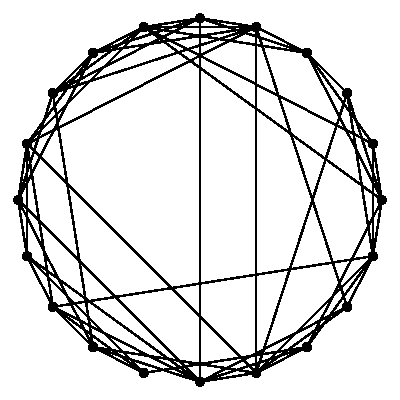
\includegraphics[width=0.4\textwidth]{WS-20-0200}
  \caption{Complex graph topology.}
  \label{c1:fig:grafos}
\end{figure}
%%%%%%%%%%%%%%%%



%Complex graphs are a special case of incomplete graphs that promote fault-tolerance while preserving a good scalability. R\'eka and Barab\'asi present an exhaustive analysis in \cite{barabasi:complex} where they prove the robust and scalable behaviour of several types of complex networks. Taking into account such properties, complex graphs interconnections are commonly used in large and unreliable architectures as they are P2P systems.

 



\clearpage
%%%%%%%%%%%%%%%%%%%%%%%%%%%%%%%%%%%%%%%%%%%%%%%%%%%%%%%%%%%%%%%%%%%%%%%%%%%%%%%
\section{Structure of the thesis}
%%%%%%%%%%%%%%%%%%%%%%%%%%%%%%%%%%%%%%%%%%%%%%%%%%%%%%%%%%%%%%%%%%%%%%%%%%%%%%%

%%%%%%%%%%%%%%%%%%
Current chapter of introduction has a descriptive orientation on the main goals and motivations behind this thesis. 
To that aim, P2P EAs are presented as an alternative for tackling large problem instances with high computing requirements whose viability will be studied in the following chapters.
%In addition, remaining sections introduce the basic working principles of Evolutionary Computation and Parallel Architectures.

%%%%%%%%%%%%%%%%%%
Chapter \ref{cap:peas} reviews the most extended models of parallel and distributed EAs and, in particular, those approaches in the literature related to P2P EAs. Besides, it provides with some insights into the role that the population structure plays on the environmental selection pressure of EAs.

%%%%%%%%%%%%%%%%%%
In chapter \ref{cap:p2pcompt}, newscast is put on the context of the current P2P platforms. Furthermore,  the protocol dynamics are assessed on the issues of decentralisation, massive-scalability and fault-tolerance.

%%%%%%%%%%%%%%%%%%
Chapter \ref{cap:model} presents the Evolvable Agent Model as the framework to evaluate the viability of the P2P EA approach. In addition, it provides some keys on the computational performance of the model and how linear speed-ups can be hold for very demanding problems in high performance computing platforms.


%%%%%%%%%%%%%%%%%%
In chapter \ref{cap:evagperformance}, the experimental analysis of the model is proposed in a simulated P2P environment so that the viability of the P2P EA can be drawn from the {\em algorithmic performance} of the approach.
Experiments are conducted for three different test-cases which focus on the algorithm scalability, the influence of the population structure in the algorithm performance and the fault-tolerance of the model for different degradation rates of the underlying computing platform.

%%%%%%%%%%%%%%%%%%
Finally, chapter \ref{cap:conclusions} exposes the main contributions of this thesis to the P2P EC area as well as possible extensions in future works.



%\s%ection{Summary}

%Evolutionary Algorithms are a set of population-based stochastic search techniques able to solve optimisation problems in reasonable time. However, for very demanding problems the execution times can be high. Parallel EAs offer an alternative to improve the algorithm performance and speed-up times to solutions. 

%In that context, we propose a P2P EA able to take full-advantage of the large amount of available resources in P2P platforms. Nevertheless, there are many challenging issues in the parallelisation of EAs in P2P systems that have to be addressed for an efficient design. Questions such as \emph{decentralisation} (such a computation paradigm is devoid of any central server), \emph{scalability} (since P2P systems  are large-scale networks) or \emph{fault tolerance} (given that resources are added and eliminated dynamically) become of the maximum interest. Therefore, the aim of this thesis is analysing our P2P EA proposal under the prisma of such issues in order to study the viability of the Peer-to-Peer Evolutionary Computation paradigm.

%In addition, this chapter presents the basic working principles of evolutionary computation and some concepts related to parallel architectures that will be used throughout the rest of the thesis.


%%%%%%%%%%%%%% Bibliografia %%%%%%%%%%%%%%%

%\bibliographystyle{alpha}  % Eliminarlo al compilar el documento maestro, ponerlo para compilarlo separado
%\bibliography{evagperformance,pea,p2pcomputing,model,methodology}%,gprop,mmitchell,zmich,hilera,fjmm,ripley,rbeale,jhertz,mag}        %Eliminarlo al compilar el documento maestro, ponerlo para compilarlo separado

%\end{document}             % Eliminarlo al compilar el documento maestro, ponerlo para compilarlo separado
